\chapter{\LaTeX 模板配置与使用}


\label{cha:sysu-thesis-latex-install-guide}

本部分内容将让你能够通过本\LaTeX 模板生成一份可用的pdf,并为后面修改源码撰写毕设做准备。

首先,我们会展示最简单的方法:直接使用overleaf进行编写。然后,我们整理了不同环境下\LaTeX 环境的配置指南与不同写作工具的配置技巧,方便各位同学使用本\LaTeX 模板。最后,我们说明了如何开始编写自己的毕业论文(设计)。


\section{使用Overleaf编写毕设}

Overleaf\footnote{网址可见\url{https://www.overleaf.com/}}是一个在线的Latex文档协作平台。我们不需要配置任何环境,便能够在上面直接使用本模板进行写作。操作步骤如下:

第一步,下载本项目压缩包(从\url{https://github.com/SYSU-SCC/sysu-thesis/releases}处下载即可),注意需要下载zip格式的压缩包。
然后,我们在Overleaf上新建项目,并上传该压缩包,可参考\autoref{fig:overleaf-new-proj}。


\begin{figure}[h]
	\centering
	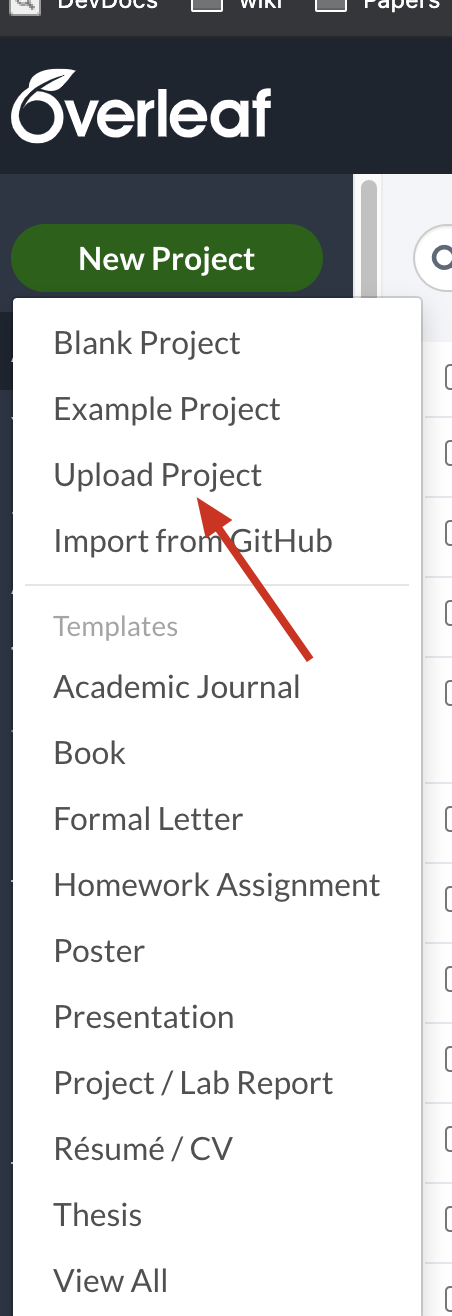
\includegraphics[width=0.2\textwidth]{image/chap03/overleaf-create-proj.jpg}
	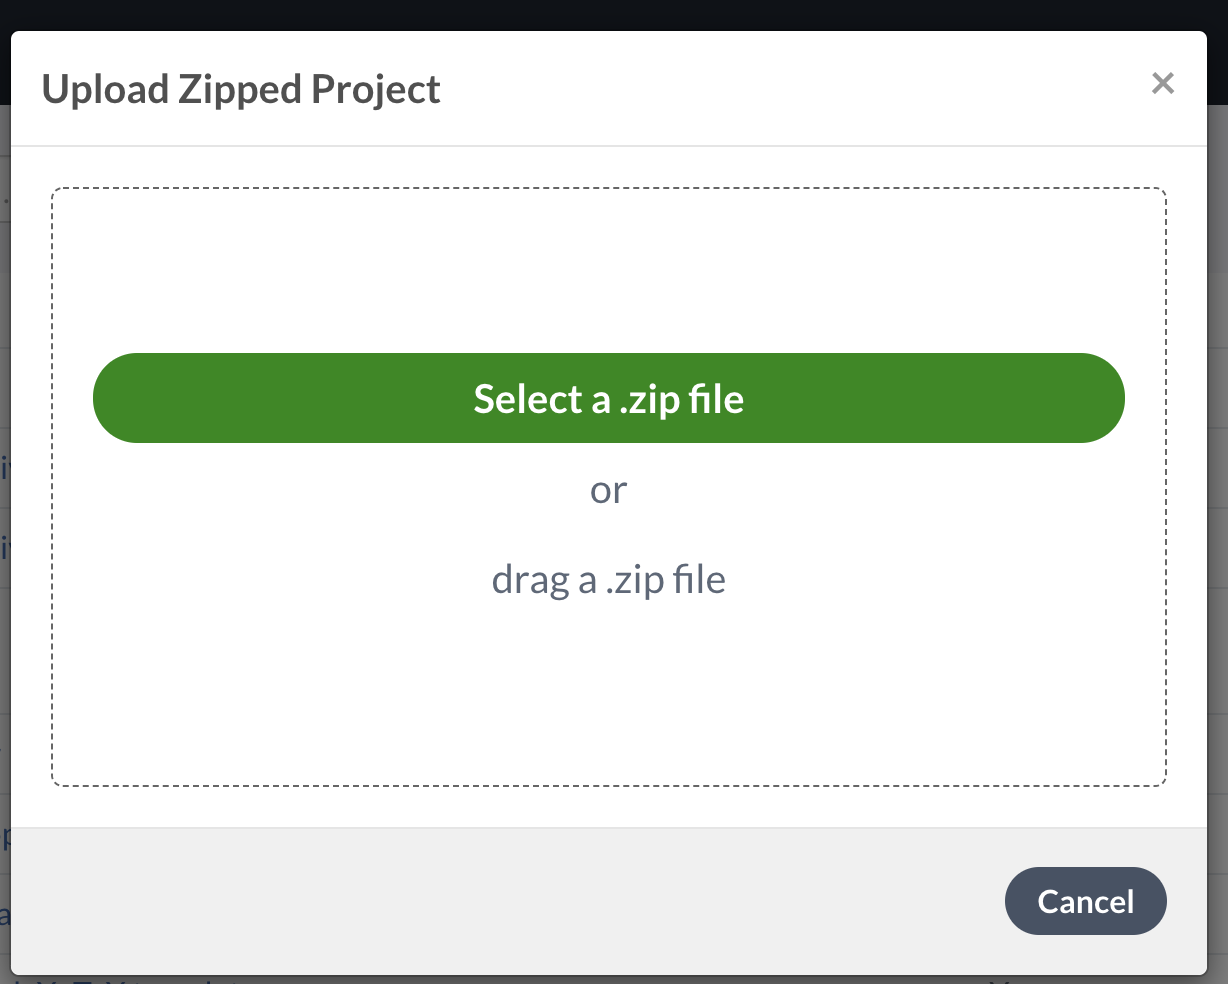
\includegraphics[width=0.7\textwidth]{image/chap03/overleaf-upload-proj.jpg}
	\caption{在Overleaf上创建并上传压缩包。}
 	\label{fig:overleaf-new-proj}
\end{figure}

第二步,在Overleaf的菜单中调整编译工具为\texttt{xelatex},可参考\autoref{fig:overleaf-config}。

\begin{figure}[h]
	\centering
	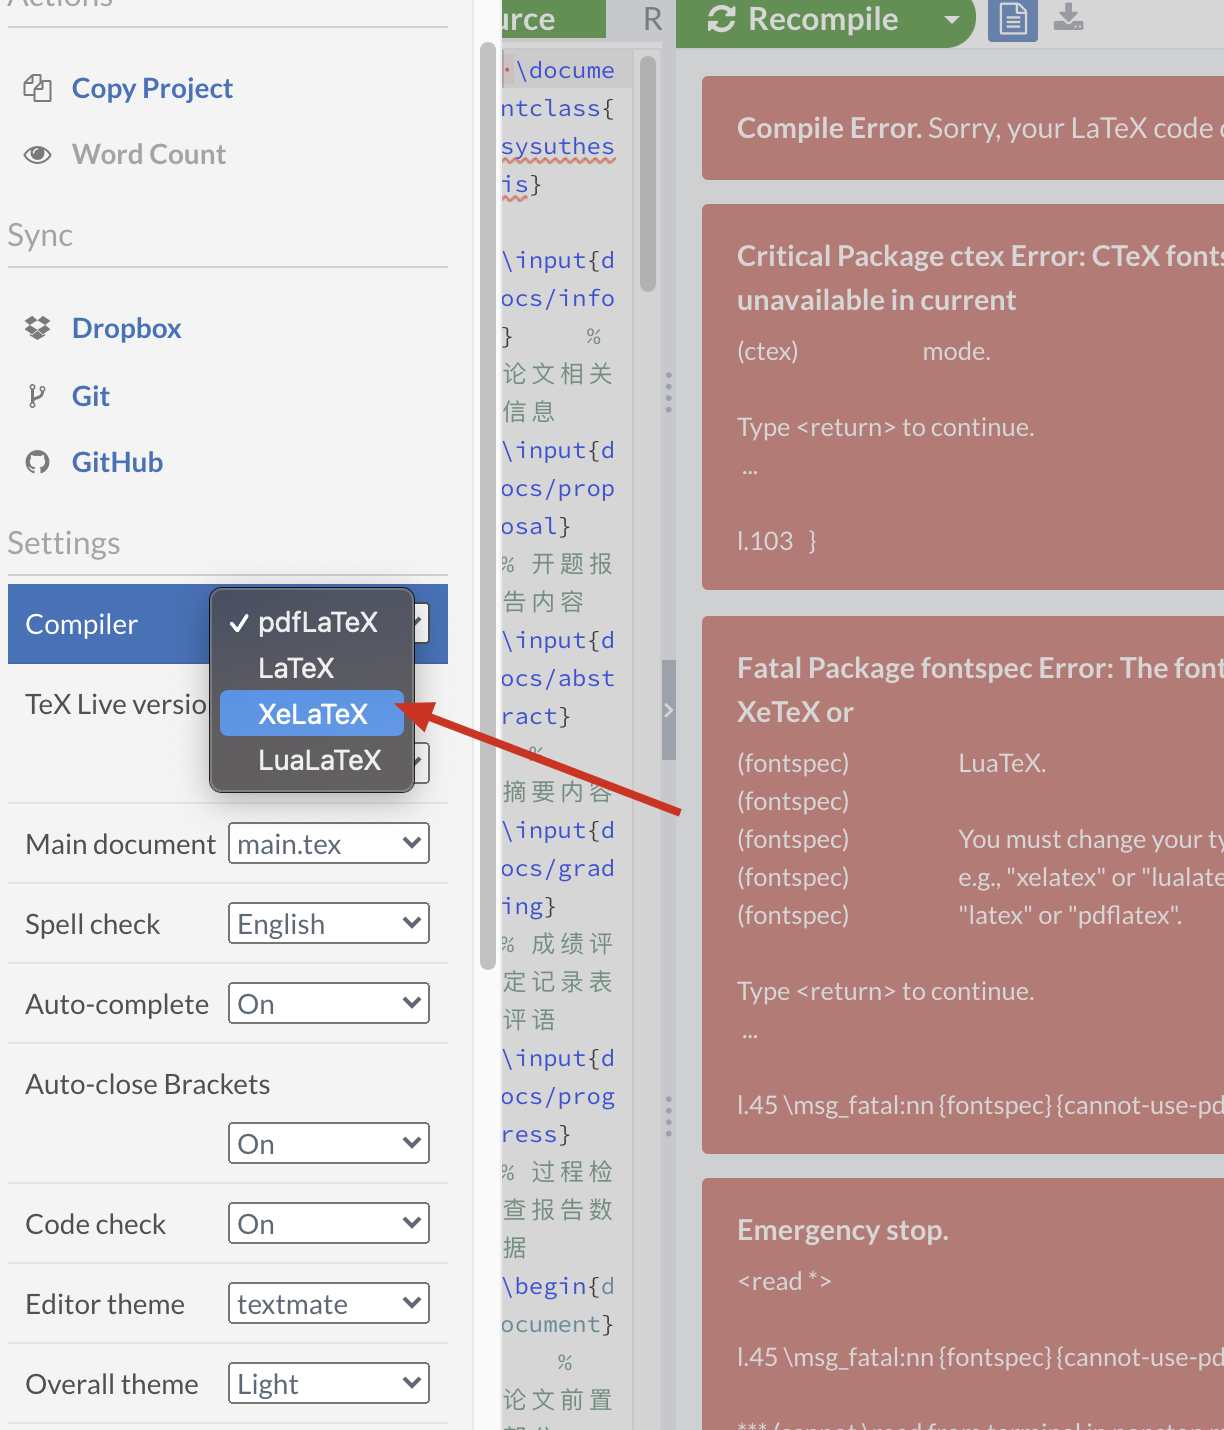
\includegraphics[width=0.6\textwidth]{image/chap03/overleaf-config.jpg}
	\caption{在Overleaf上调整编译工具}
 	\label{fig:overleaf-config}
\end{figure}


第三步,点击编译,得到本pdf,可以开始修改pdf了!最终可见\autoref{fig:overleaf-example}。


\begin{figure}[h]
	\centering
	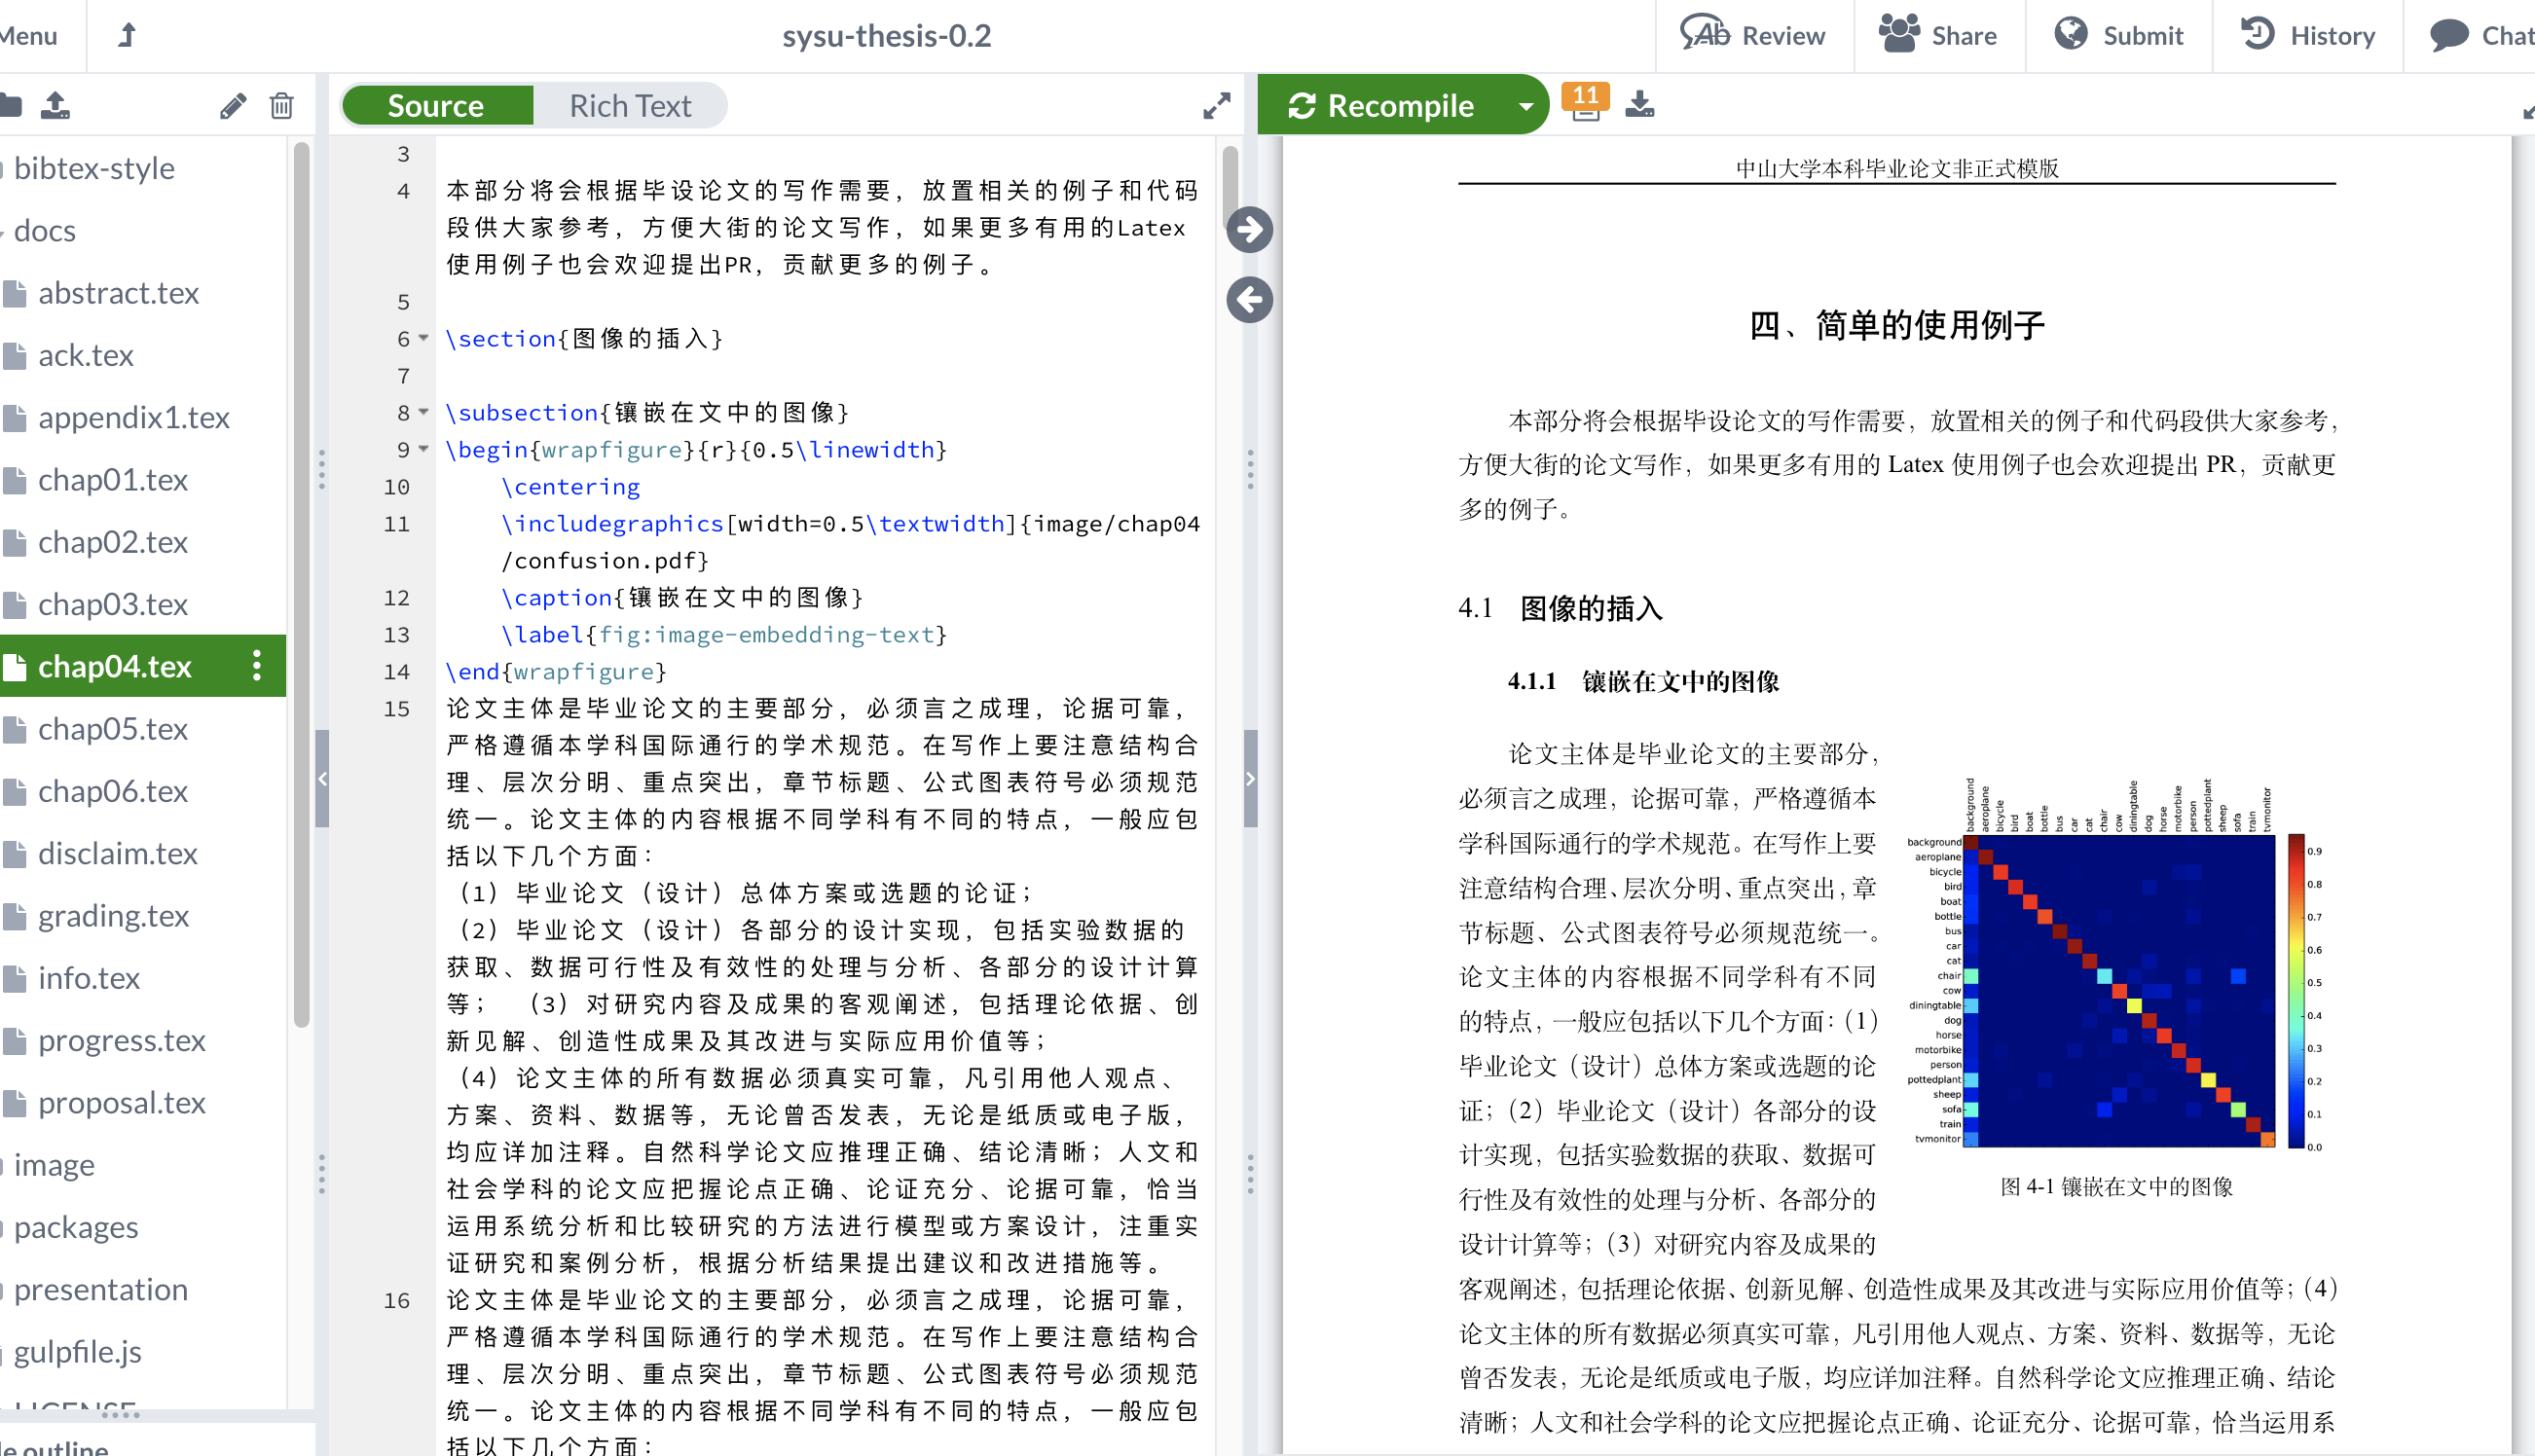
\includegraphics[width=0.9\textwidth]{image/chap03/overleaf-example.jpg}
	\caption{Overleaf使用例子}
 	\label{fig:overleaf-example}
\end{figure}



\section{编译环境配置}

编译环境配置相对来说比较简单,下载Tex Live2020并如同一般的程序一样安装即可。

\subsection{编译环境配置:Window篇}

在\url{https://mirrors.tuna.tsinghua.edu.cn/CTAN/systems/texlive/Images/}上下载Tex Live2020并参考教程\footnote{可以参考\url{https://zhuanlan.zhihu.com/p/58811994}}安装即可。

\subsection{编译环境配置:Linux篇}

在\url{https://mirrors.tuna.tsinghua.edu.cn/CTAN/systems/texlive/Images/}上下载Tex Live2020并参考教程\footnote{可以参考\url{https://zhuanlan.zhihu.com/p/55894177}}安装即可。


\subsection{编译环境配置:MacOS篇}

在MacOS上配置Latex的环境,这里我们使用的是MacTex。

\begin{enumerate}
    \item \url{https://www.tug.org/mactex/}下载MacTex安装。
    \item 安装步骤:不详细展开,按照图形界面点击即可, 傻瓜式安装。
\end{enumerate}

TIPS:MacTex文件比较大,有2G多,介意的话可以选择MacTex\_Basic包,只有100M以内,但是如果安装MacTex\_Basic,后期可能会遇到各种缺包的问题。


安装完成之后,可以简单测试一下安装是否成功。如可以查看Texshop应用是否安装好,或者在命令行测试一下\texttt{xelatex}命令是否可用。

\section{写作环境配置}

不同的写作工具对应不同的写作环境。这里我们给出几个工具的配置例子以供参考。

\subsection{模板编译流程}

由于\LaTeX 的限制,本模板需要经过四次编译才能生成完整的论文:

\begin{enumerate}
    \item 先使用xelatex编译一次
    \item 再使用bibtex编译一次
    \item 然后使用xelatex编译两次
\end{enumerate}

本编译流程已经写在Makefile中,修改模板源码后只需要执行\texttt{make pdf}即可按照该流程进行编译并生成最终的pdf。



\subsection{写作环境配置:Visual Studio Code}

Visual Studio Code是微软公司推出的轻量代码编辑器,我们可以做一些简单的配置,便可以用该编辑器修改我们的\LaTeX 模板,并实现一键编译。

\begin{enumerate}
    \item 安装 Visual Studio Code。
    \item 安装 LaTeX Workshop 插件。
\end{enumerate}

本项目的\texttt{.vscode/setting.json}下已经包含了与前面所述编译流程相同的配置。正常配置下,每次修改模板源码后按下保存(Ctrl+S),就能够自动进行编译产生pdf。效果图如\autoref{fig:vscode-example}所示。


\begin{figure}[h]
	\centering
	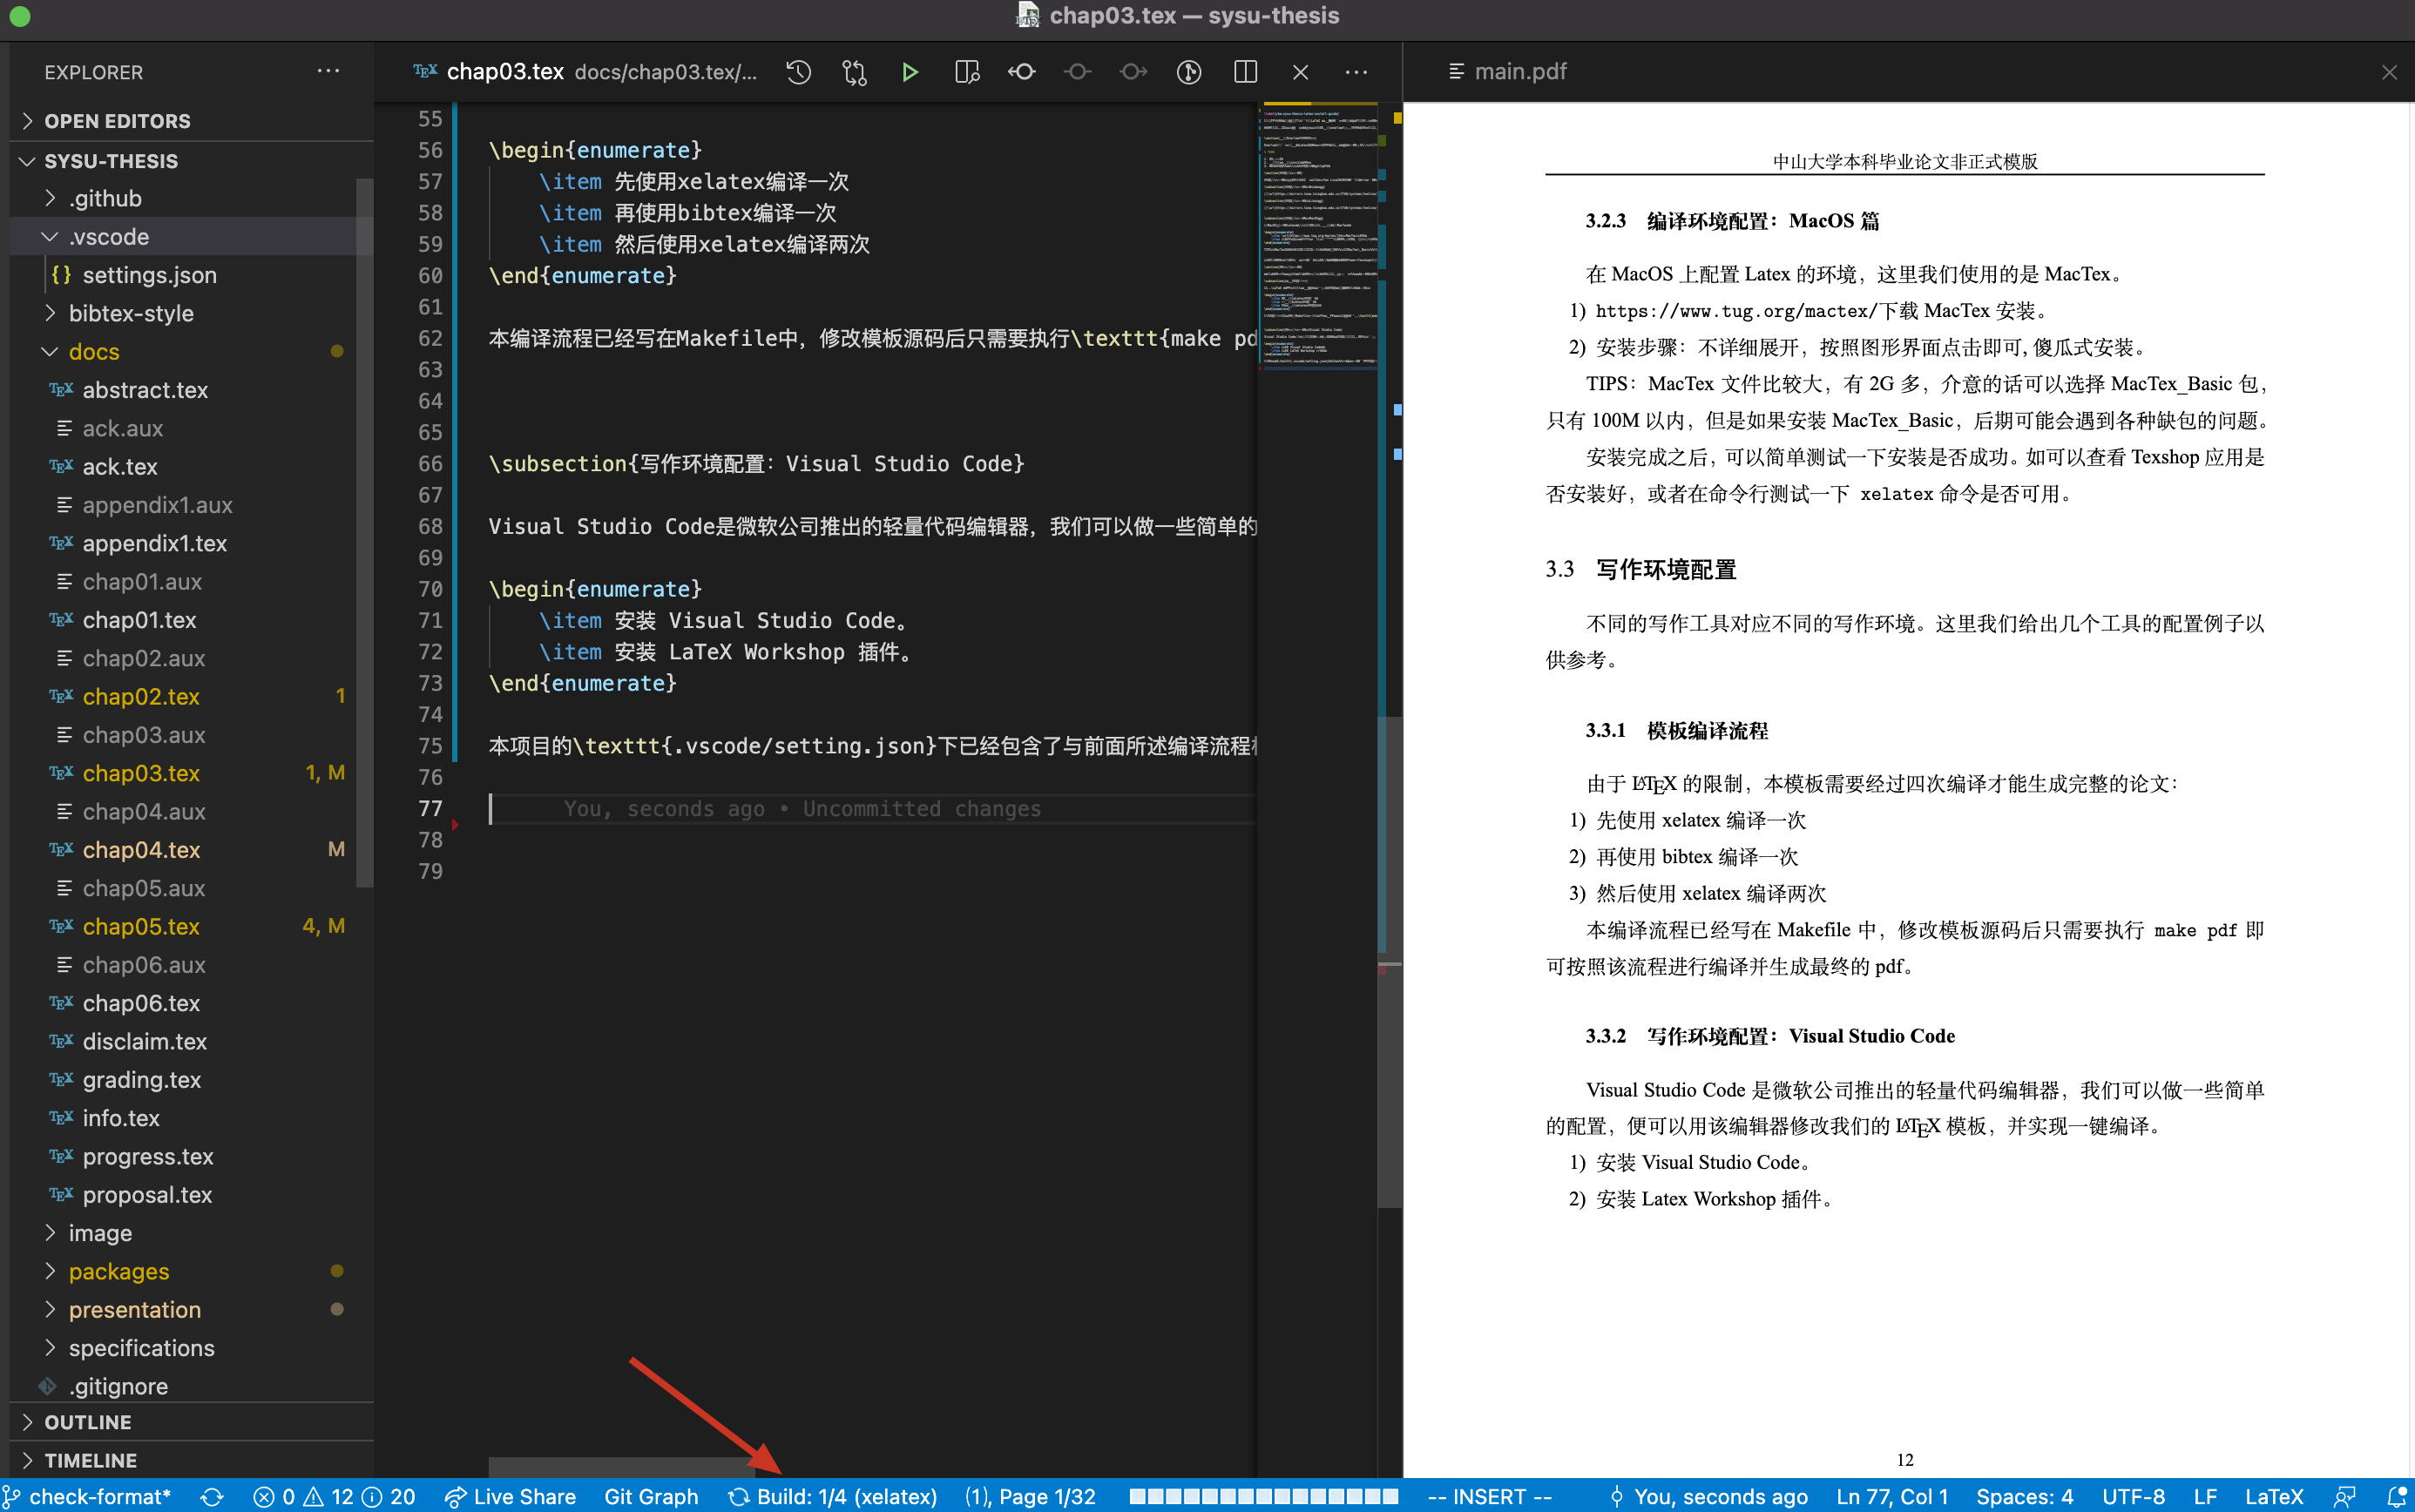
\includegraphics[width=\linewidth]{image/chap03/vscode-example.png}
	\caption{vscode配置好后的样例}
 	\label{fig:vscode-example}
\end{figure}


\section{如何开始写毕业论文(设计)}

首先将所有个人信息,包括学号、姓名、专业、论文题目等,在\texttt{./docs/info.tex}中逐项进行更新。

然后我们再编辑\texttt{./docs/abstract.tex}补充论文摘要。

到了论文主体部分,我们可以自行编辑\texttt{./docs/chap01.tex},\texttt{./docs/chap02.tex}等文件进行编辑。如果章数不够,可以自行修改\texttt{main.tex}增加新的章节。

当论文主体编写完成后,我们再编辑\texttt{./docs/ack.tex}作为论文致谢。


% 首先将个人信息写到\texttt{./docs/info.tex}中。